\section{Dokumentation der Implementierung}

% Sollte größter Teil werden
% - High level overview?
% - Wie läuft das auf meinem System?
% - Code Dokumentation / Entwicklerdokumentation

%%%%%%%%
% Highlevel
% ca 1-2 Seiten
% Buzzwords, grober Überriss

%%%%%%%%
% Middle level
% ca 2-3 Seiten
% Skripte, libraries/packages, Setup
% beispielbilder /output
% getestete Systeme (ARM/Raspi, Debian stretch, x86)
% mindeste was in README.md im master liegen sollte
% viel bereits in READMEs der zugehörigen Ordner zusammengefasst
% backend-deployment -> Niels
% frontend-deployment -> Max

%%%%%%%%
% Low level
% was muss ich als entwickler wissen
% tiles, parallelisierung, structs/klassen, struktur des projekts

% Zuordnung klasse -> Dokumentation
% backend
%   *.main.cpp, init -> Niels DONE
%   include Ordner und CMake -> Niels DONE
%   balancer + tests -> Florian
%   mandelbrot -> Florian (außer MandelbrotSIMD -> Niels DONE)
%   actors
%      Worker -> Tobi
%      Host
%         websocket-funktionen -> Niels
%         Rest -> Tobi
%           + Parallelisierungskonzept (+ welche MPI Method, warum)
%   structs/Netzwerk -> Tobi/Niels/Florian
%   dev-environment (was ist docker und wie/warum) -> Max
% frontend
%    connection -> Niels
%    tileDisplay -> Max
%        TileDisplay.ts
%            Prinzip 
%            genauer Ablauf/Funktionen
%               + Shader
%        WorkerLayer.ts
%           + Gruppierung
%        MatrixView.ts + RegionOfInterest.ts
%        Project.ts
%    visualization -> Niels
%    misc -> Max

%%%%%%%%%%%%%%%%%%%%%%%%%%%%%%%%%%%%%%%%%%%%%%%%%%
% Abschnitt - Grober Überblick
%%%%%%%%%%%%%%%%%%%%%%%%%%%%%%%%%%%%%%%%%%%%%%%%%%

\subsection{Überblick}

% TODO Ein bisschen mehr details
Das Problem fordert eine Unterteilung in drei wesentliche Bausteine, wie sie in \autoref{fig:architekturuebersicht} zu sehen sind.
Eine Benutzeroberfläche in einem Web Browser des Benutzers (“Frontend”), welches die Benutzerinteraktionen entgegennimmt und mit dem Backend kommuniziert.
Ein Backend-Host übernimmt dazu die Kommunikationsfunktion, verwaltet die eingehenden Rechenaufträge und verteilt sie an die Backend-Worker. Das Ergebnis dieser Berechnung sendet der Host dann an das Frontend zurück.
Die Backend-Worker nehmen die zugewiesenen Rechenaufträge entgegen und führen die eigentlichen Berechnungen verteilt aus.

\begin{figure}
    % Bindet das als PDF exportierte pptx ein -> vektorgrafik
    % -> pptx bearbeiten statt pdf
    \centering
        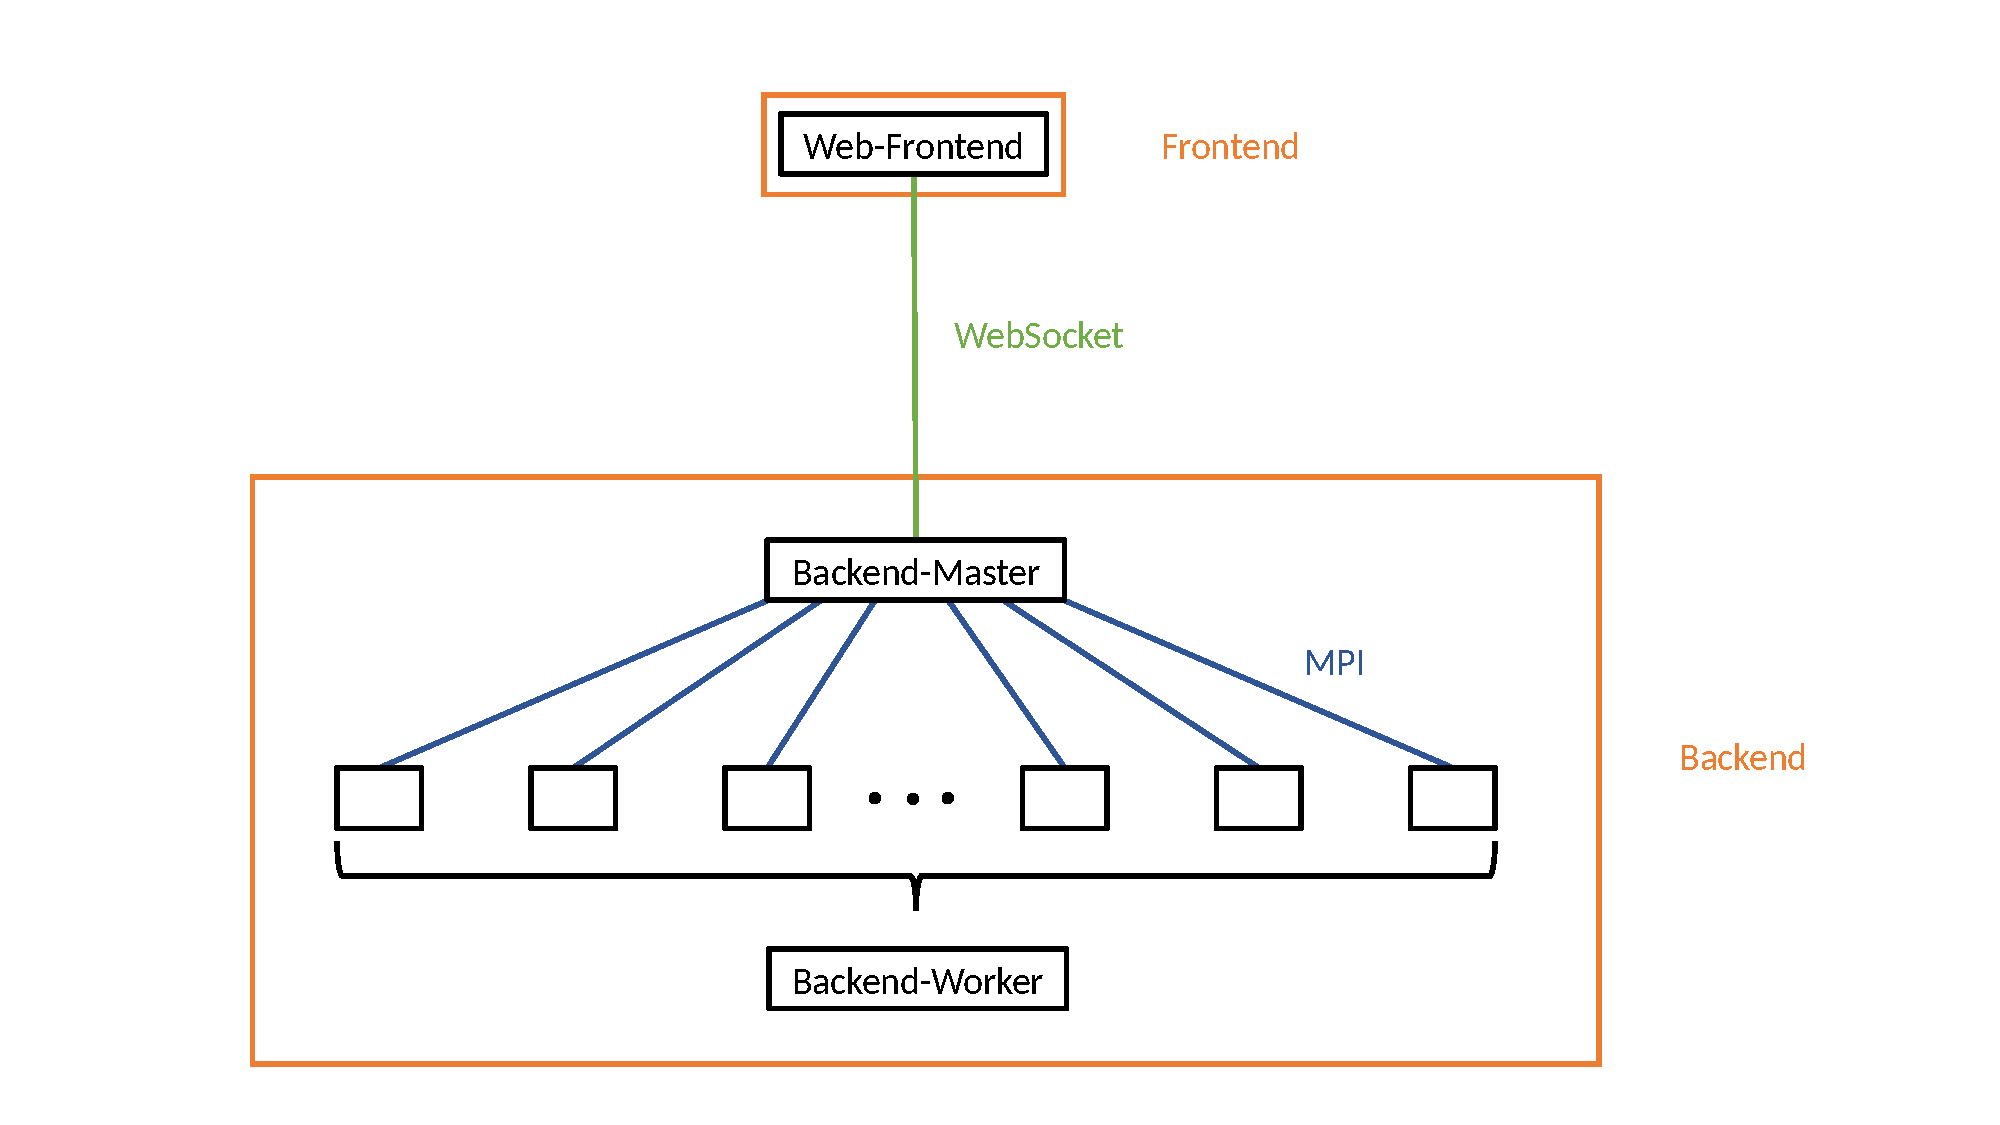
\includegraphics[width=0.98\linewidth]{img/Implementierung/Kommunikation.pdf}
        \caption{Architekturübersicht}
    \label{fig:architekturuebersicht}
\end{figure}

\subsection{Aufsetzen des Backends}

\subsubsection{Schnellstart}

Um das System schnell zum laufen zu bekommen, muss das Repository auf das eigene System geklont werden.
Im Unterverzeichnis
=> README aus backend/himmuc übertragen

\subsection{Implementierung der Mandelbrotberechnung}

Zur hardwarenahe Berechnung der Mandelbrotmenge wird ein sogenanntes Backend gestartet.
Das in C++ programmierte Teilprojekt nimmt Rechenaufträge von einem Nutzer durch ein Frontend entgegen (auch
ein solches wird bereitgestellt), zerlegt sie und verteilt sie per MPI auf dedizierte Rechenknoten.
Dazu besteht das Backend aus zwei ausführbaren Dateien, host und worker. % Code-mäßiges highlighten möglich??

\subsubsection{Inkludierte Header und CMake Anweisungen}

Die zusammenstellung der ausführbaren Dateien wird in CMake definiert.
Dabei unterscheiden sich diese lediglich in den eingebundenen Quelldateien:
In die Datei host werden host.main.cpp und actors/Host.cpp eingebunden, während
in worker worker.main.cpp und actors/Worker.cpp eingebunden werden.

Diese und alle weiteren Build-Vorgaben werden in der Datei CMakeLists.txt für 
cmake\footnote{Ein Programm, welches die Erstellung von Makefiles vereinfacht in dem es sie automatisch an die Umgebung des Build-Systems anpasst. \url{https://cmake.org/}}
in der hier beschriebenen Reihenfolge spezifiert.

Es sollte hierbeit eine CMake-Version über 3.7.0 gewählt werden und die C++11 Standarts\footnote{\url{https://isocpp.org/wiki/faq/cpp11}} werden vorrausgesetzt.
Zudem werden für das Projekt "Mandelbrot" werden alle Dateien im Order include eingebunden.
In diesem Ordner liegen die Header-Dateien für alle projektinternen C++-Quelldateien.
Anschließend werden alle C++-Quelldateien (Endung ".cpp") aus dem Ordner src in einer Liste gesammelt, mit Ausnahme jedoch der oben genannten, exklusiven Quelldateien.
Die erzeugte Liste und die jeweils exklusiven Dateien werden dann den ausführbaren Dateien host und worker zugeordnet.

Um die verwendeten Biblioteken verfügbar zu machen werden anschließend die Header der installierten MPI-Bibliotek
sowie die Header der Bibliotheken rapidjson\footnote{\url{http://rapidjson.org}}, websocketpp\footnote{\url{https://github.com/zaphoyd/websocketpp}} und boost\footnote{\url{https://www.boost.org/}}
Diese werden respektive verwendet um JSON zu parsen und enkodieren, Websocket-Verbindungen aufzubauen und darüber zu kommunizieren sowie um diese Bibliothek zu unterstützen.
Da für die boost Bibliothek dabei Header nicht genügen und die systemweite Verfügbarkeit der kompilierten boost-Bibliothek nicht garantiert werden kann, wird die Teilbibliothek boost\_system statisch
in die ausführbaren Datei host eingebunden.

Zuletzt werden über Compilerflags alle Kompilierfehler und -warnungen aktiviert sowie die POSIX-Thread-Bibliothek eingebunden
und spezielle Flags für die Websocketlibrary und MPI gesetzt.

\subsubsection{Mainfunktion und Initialisierung}

Zur Initialisierung der Prozesse muss zunächst die MPI-Umgebung aktiviert und abgerufen werden.
Dies geschieht für beide Programme gleich, über die Initialisierungsfunktion in \autoref{src:init.cpp}.
Sie erwartet lediglich eine Beschreibung des Prozesses für den Log und eine Initialisierungsfunktion,
die erst zurückkehrt, wenn das Programm abgeschlossen ist und MPI beendet werden soll.
Die Funktion muss als Parameter den Rang bzw. die Id des aktuellen MPI-Prozesses und die Anzahl der initialisierten
Prozesse entgegen nehmen.

Ein beispielhafter Aufruf ist in \autoref{src:host.main.cpp} zu sehen. Damit wird MPI initialisiert und nach der
erfolgreichen Initialisierung der eigentliche \hyperref[cls:Host]{Host-Prozess} über Host::init gestartet.

\begin{figure}
    \lstinputlisting[caption={Initialisierung der MPI-Prozesse in init.cpp}, label={src:init.cpp}, firstline=15, lastline=39, firstnumber=15]{../../backend/src/init.cpp}
\end{figure}


\begin{figure}
    \lstinputlisting[caption={Initialisierung des Host-Prozesses in host.main.cpp}, label={src:host.main.cpp}]{../../backend/src/host.main.cpp}
\end{figure}

\subsection{Host Funktionalitäten} \label{cls:Host}

\subsubsection{Websocketverbindung}

Direkt nach der Initialisierung des Host-Programmes in \autoref{src:Host.cpp::init.websocket}, wird ein separater Thread gestartet, der über Websocket
Anfragen zur Berechnung einer Region entgegennimmt und ein Thread, der berechnete Regionen an den verbundenen Client übergibt.

\begin{figure}
    \lstinputlisting[caption={Starten des Websocketservers bei der Initialisierung des Host-Programmes in Host.cpp}, label={src:Host.cpp::init.websocket}, firstline=387, lastline=398, firstnumber=387]{../../backend/src/actors/Host.cpp}
\end{figure}

\subsection{Lastbalancierung}
Um die Mandelbrotmenge effizient parallel zu berechnen, muss die Last gleichmäßig auf die Worker verteilt werden.
Die Aufgabe der Lastbalancierung besteht darin zu einer gegebenen Region und einer Anzahl von Workern eine solche Unterteilung in sogenannte Teilregionen zu finden.
Wichtig dabei ist, dass der garantierte Teiler von Höhe und Breite der Teilregionen dem der angeforderten Region entspricht, da es sonst im Frontend zu Schwierigkeiten bei der Darstellung kommt.
Die Klassenstruktur der Lastbalancierer entspricht dem Strategy-Pattern. So kann der Balancierer zur Laufzeit leicht gewechselt werden und auch die Erweiterung des Projekts um eine weitere Strategie gestaltet sich einfach.
Was dabei genau beachtet werden muss findet sich im Teil \hyperref[lastbalancierung_erweiterung]{Erweiterung}.


Damit die Unterschiede zwischen guter und schlechter Lastverteilung deutlich werden, wurden hier verschiedene Strategien zur Lastbalancierung implementiert.

\subsubsection{Naive Strategie}

Bei der naiven Strategie (zu finden in den Klassen NaiveBalancer und RecursiveNaiveBalancer) wird versucht den einzelnen Workern etwa gleich große Teilregionen zuzuweisen.
Dies geschieht allerdings ohne Beachtung der eventuell unterschiedlichen Rechenzeiten innerhalb der Teilregionen.
Die naive Strategie wurde hier in einer nicht-rekursiven  und einer rekursiven Variante implementiert.

\paragraph*{} \label{lastbalancierung_naiv}
%non-recursive naive
Zur nicht-rekursiven Aufteilung wird zuerst die Anzahl der zu erstellenden Spalten und Zeilen berechnet.
Dazu wird der größte Teiler der Anzahl der Worker bestimmt. Dieser gibt die Anzahl der Spalten an, das Ergebnis der Division ist die Anzahl der Zeilen.
Damit ist sichergestellt, dass die Region in die richtige Menge von Teilregionen unterteilt wird.

Als nächstes wird die Breite und Höhe der Teilregionen berechnet. Hierbei ist wichtig, dass der garantierte Teiler erhalten wird.
Die Breite berechnet sich also durch:
\begin{equation*}
	\frac{region.width}{region.guaranteedDivisor * nodeCount} * region.guaranteedDivisor
\end{equation*}
Dabei ist $nodeCount$ die Anzahl der Worker und $region$ die zu unterteilende Region.
Es ist zu beachten, dass es sich hier um eine Ganzzahldivision handelt, deren Rest angibt, wie viele Teilregionen um $region.guaranteedDivisor$ breiter sind.
Die Höhe berechnet sich analog.

Bevor die eigentliche Aufteilung beginnt werden noch die Deltas für Real- und Imaginärteil bestimmt.
Diese geben an, wie breit bzw. hoch der Bereich der komplexen Ebene ist, den ein Pixel der Region überdeckt.
Die Deltas können über Methoden der Klasse Fractal berechnet werden.

Zur Aufteilung wird nun mittels zweier verschachtelter Schleifen über die Zeilen und Spalten iteriert.
Die benötigten Start- und Endpunkt der Teilregionen (also die linke obere Ecke und die rechte untere Ecke auf der komplexen Ebene) können nun mithilfe der Schleifenzähler und der Deltas bestimmt werden.
Zusätzlich wird noch der vertikale und horizontale Offset der Teilregion vom Startpunkt der Eingaberegion abgespeichert. Diese Information ermöglicht es die Region im Frontend einfach anzuzeigen.

Falls die aktuell betrachtete Teiregionen zu den Breiteren und/oder Höheren (s.o.) gehört, müssen alle Werte entsprechend angepasst werden.
Die letzte Teilregion einer Spalte bzw. Zeile wird immer so gewählt, dass sie auf jeden Fall mit dem Rand der Eingaberegion abschließt.

Die Teilregionen werden in einem Ergebnisarray gespeichert, welches dann zurückgegeben wird.

\paragraph*{} \label{lastbalancierung_naiv_rekursion}
% recursiveNaive
Die Grundidee der rekursiven Balancierung ist, die Region solange zu halbieren, bis man genug Teile für jeden Worker hat.
Dies funktioniert sehr gut, wenn die Anzahl der Worker eine 2er-Potenz ist. Wenn das nicht der Fall ist, so müssen für einige Worker die Regionen öfters geteilt werden als für andere.
Die Anzahl der Blätter des Rekursionsbaumes (hier ein Binärbaum) muss also der Anzahl der Worker entsprechen.
Die Rekursionstiefe kann man wie folgt berechnen:
\begin{equation} \label{lastbalancierung_rekursion_tiefe}
	recCounter = \lfloor\log_2 nodeCount\rfloor + 1
\end{equation}
Und die Anzahl der Teilregionen auf der untersten Ebene des Rekursionsbaumes ergibt sich als:
\begin{equation*}
	missing = nodeCount - 2^{\lfloor\log_2 nodeCount\rfloor}
\end{equation*}
\begin{equation} \label{lastbalancierung_rekursion_ebene}
	onLowestLevel = missing * 2
\end{equation}
Auch hier ist $nodeCount$ die Anzahl der Worker. Die Multiplikation mit 2 ist nötig, da nochmal $missing$ Blätter aufgeteilt werden müssen, um $missing$ zusätzliche Blätter zu erzeugen.

Um diese Werte einfach durch die Rekursionsebenen zu reichen wurde die Struktur BalancingContext definiert, welche zusätzlich noch die beiden Deltas, den Index in das Ergebnisarray und einen Zeiger auf das Array selbst abspeichert.

Aus $recCounter$ und $onLowestLevel$ kann auch die Abbruchbedingung der Rekursion gefolgert werden:
\begin{equation} \label{lastbalancierung_rekursion_abbruch}
	recCounter = 0 \vee (recCounter = 1 \wedge resultIndex \geq onLowestLevel) \equiv true
\end{equation}
$resultIndex$ ist hierbei der Index in das Ergebnisarray, beschreibt also die Anzahl der bereits erstellten Teilregionen.

Ist die Abbruchbedingung (\ref{lastbalancierung_rekursion_abbruch}) erfüllt, so genügt es die übergebene Region in das Ergebnisarray einzutragen und $resultIndex$ zu inkrementieren.
Ansonsten muss die Region halbiert werden. Ist die Region vertikal oder horizontal nicht mehr teilbar (d.h. $region.width$ bzw. $region.height$ $\leq region.guaranteedDivisor$), so wird in die andere Richtung geteilt.
Kann die Region in beide Richtungen geteilt werden, so wird abwechselnd vertikal und horizontal geteilt. Dies gewährleistet, dass der Balancierer in beide Richtungen aufteilt, sofern das möglich ist.
Wenn die Region unteilbar ist, so muss eine leere Region erzeugt werden.

Die beiden Hälften berechnen sich wie bei der Aufteilung auf zwei Worker mit der \hyperref[lastbalancierung_naiv]{nicht-rekursiven Strategie}.
Dann wird die Funktion für jede Hälfte rekursiv aufgerufen.

\subsubsection{Strategie mit Vorhersage}

Bei dieser Strategie (zu finden in den Klassen PredictionBalancer und RecursivePredictionBalancer) basiert die Aufteilung der Region auf einer Vorhersage über die Rechenzeit.
Die Teilregionen werden so gewählt, dass sie, entsprechend der Vorhersage, etwa einen ähnlichen Rechenaufwand haben.

Die Vorhersage (struct Prediction) wird von der Klasse Predicter angestellt.
Dazu wird die Region in einer sehr viel geringeren Auflösung berechnet.
Die benötigte Anzahl an Iterationen wird jeweils pro Kachel (Breite und Höhe sind der garantierte Teiler) abgespeichert.
So wird sichergestellt, dass der garantierte Teiler auch nach der Aufteilung noch gilt, da die Balancierer die Vorhersage Eintrag für Eintrag verarbeiten.
Die Genauigkeit der Vorhersage kann über das Attribut $predictionAccuracy$ gesteuert werden:
\begin{itemize}
	\item $predictionAccuracy > 0$: $(predictionAccuracy)^2$ Pixel werden pro Kachel berechnet. Die Summe der Iterationen für die einzelnen Pixel ergibt die Vorhersage für die Kachel.
	\item $predictionAccuracy < 0$: Für $(predictionAccuracy)^2$ Kacheln wird ein Pixel in der Vorhersage berechnet. Es erhalten also mehrere Kacheln diesselbe Vorhersage.
	\item $predictionAccuracy = 0$: Unzulässig, es wird ein Null-Pointer zurückgegeben.
\end{itemize}
Es ist wichtig eine gute Balance zwischen Güte und Geschwindigkeit der Vorhersage zu finden.
Zusätzlich beinhaltet die Vorhersage die Summen der benötigten Iterationen pro Spalte und Zeile, sowie die Gesamtsumme.
Auch die Deltas für Real- und Imaginärteil pro Kachel und die Anzahl der Zeilen und Spalten werden angegeben.

Auch die Strategie mit Vorhersage wurde in einer rekursiven und in einer nicht-rekursiven Variante implementiert.

\paragraph*{} \label{lastbalancierung_vorhersage}
% non-recursive prediction
Für die nicht-rekursive Variante wird zuerst die benötigte Anzahl an Zeilen und Spalten bestimmt.
Dies geschieht genauso wie bei der naiven Strategie.

Die erzeugten Teilregionen sollen in etwa den gleichen Rechenaufwand haben. Dieser berechnet sich durch:
\begin{equation} \label{lastbalancierung_vorhersage_formel}
	desiredN = \frac{nSum}{nodeCount}
\end{equation}
Dabei ist $nSum$ die Gesamtsumme der Vorhersage und $nodeCount$ wieder die Anzahl der Worker.

Danach wird die Region erst in Spalten aufgeteilt und in einem zweiten Schritt wird dann die horizontale Unterteilung in Teilregionen vorgenommen. 

Zur Aufteilung wird über die Spaltensummen in der Vorhersage iteriert. Diese werden aufaddiert und bilden so den Zähler $currentN$.
Sobald $currentN$ $\geq desiredN$ gilt oder für alle restlichen Spalten nur noch je ein Eintrag in den Spaltensummen vorhanden ist, wird eine Spalte abgeschlossen.
Dazu werden $maxReal$ und $width$ aus den Zählern berechnet. Es ist wichtig $maxReal$ immer neu aus $region.minReal$ zu berechnen, anstatt nur das Delta aufzuaddieren, da sich sonst der Fehler, der bei Fließkommaaddition unvermeidbar ist, auch mit aufaddiert. $minReal$ und $hOffset$ stehen bereits in $tmp$, die Werte wurden bei der Berechnung der vorhergehenden Spalte bereits gesetzt.
Jetzt wird $tmp$ für die nächste Spalte vorbereitet, das heißt $tmp.minReal$ wird auf $tmp.maxReal$ gesetzt und $tmp.hOffset$ wird um $tmp.width$ erhöht. Ersteres vermeidet das Entstehen von Lücken zuverlässig.
Außerdem wird $desiredN$ für die verbleibenden Spalten nach (\ref{lastbalancierung_vorhersage_formel}) neu berechnet und die Zähler werden zurückgesetzt.
Bevor die Aufteilung der Spalte in Teilregionen startet, wird eine Kopie der Vorhersage erstellt, die nur die Werte für die aktuelle Spalte enthält.
Das Aufteilen einer Spalte in Teilregion geschieht analog zum Aufteilen in Spalten.

Die letzte Spalte wird gesondert behandelt: Sie muss so gewählt werden, dass sie den gesamten Rest der Eingaberegion abdeckt, ansonsten können Lücken entstehen.
Dies gilt genauso bei der Unterteilung der einzelnen Spalten.

\paragraph*{}
% recursive prediction
Die rekursive Variante der Strategie mit Vorhersage verwendet dasselbe Rekursionsschema wie ihr \hyperref[lastbalancierung_naiv_rekursion]{naives Gegenstück}.
Die Werte in BalancingContext berechnen sich also wie in (\ref{lastbalancierung_rekursion_tiefe}) und (\ref{lastbalancierung_rekursion_ebene}).
Auch die Abbruchbedingung ist wie in (\ref{lastbalancierung_rekursion_abbruch}). Die Entscheidung, ob horizontal oder vertikal geteilt werden soll, wird auch auf die gleiche Art und Weise gefällt.

Bei dieser Strategie werden die Regionen allerdings nicht einfach halbiert, sondern in zwei Teile aufgeteilt, die laut der Vorhersage ähnlich rechenintensiv sind.
Dazu wird so vorgegangen, wie bei der \hyperref[lastbalancierung_vorhersage]{nicht-rekursiven Variante} für die Aufteilung auf zwei Worker.
Es ist hierbei auch wichtig die Vorhersage so zu teilen, dass es für jede Hälfte eine Vorhersage gibt, die dann an den rekursiven Aufruf übergeben werden kann.

\subsubsection{Leere Regionen} \label{lastbalancierung_leereregion}

\subsubsection{Erweiterung} \label{lastbalancierung_erweiterung}

\subsection{Berechnung der Mandelbrotmenge}

\subsubsection{Berechnung mithilfe von SIMD}

Um die Berechnungen intern noch zu beschleunigen, kann SIMD zur parallelen Bearbeitung mehrerer Punkte verwendet werden.
Dazu ist es hilfreich, sich zunächst vor Augen zu führen, wie ein Vektor komplexer Koordinaten ohne SIMD verarbeitet würde.
Dies ist in \autoref{src:MandelbrotVect.cpp} zu sehen.
Die Berechnung der einzelnen Kooridnaten bleibt gleich, nur die Abbruchbedingung wird auf alle bearbeiteten Koordinaten erweitert.

Es muss dabei solange weiter iteriert werden, bis für alle Komponenten die Berechnung abgebrochen werden darf.
Hierbei ist es kein Problem, mit den abgebrochenen Punkten weiter zu rechnen, sofern die 
Iterationszahl nur hochgezählt wird solange das $z_n$ der Koordinate Betragsmäßig kleiner gleich $2$ ist.
Dies gilt, da alle $|z_{n+i}| > 2$ sofern $|z_n| > 2$ \cite{424331}.

\begin{figure}
    \lstinputlisting[caption={Bearbeitung eines Vektors komplexer Koordinaten in C++}, label={src:MandelbrotVect.cpp}, firstline=8, lastline=46, firstnumber=8]{../../backend/src/mandelbrot/MandelbrotVect.cpp}
\end{figure}

Damit kann die Berechnung relativ simpel via Arm NEON Compiler Intrinsics\footnote{Details im Abschnitt "Compiler Intrinsics" unter \url{https://developer.arm.com/technologies/neon}} implementiert werden (siehe dazu \autoref{src:MandelbrotSIMD32.cpp}).
Diese Intrinsics ermöglichen eine Verwendung der nativen SIMD-Befehle, wobei der Compiler sich um die Verwendung der SIMD-Register kümmert.
Dadurch wird lesbarer Code ermöglicht, der sich stärker am zu implementierenden Algorithmus orientiert.

Zu den hier benötigten mathematischen Operationen (z.B. der Addition) wird hierbei das Compiler Intrinsic nach folgendem Schema erzeugt:
"v\textit{opc}q\_f\textit{pr}" mit dem Operationscode \textit{opc} (z.B. \textit{add} für Addition).
"v" ist das allgemeine Prefix für Vektoroperationen und "q" bedeutet, dass doppelt so viele Register verwendet werden wie ohne "q".
Damit werden alle verfügbaren SIMD-Register des ARMv8-A Prozessors des ODroids und Raspberry Pi 3 B+ herangezogen.
Das Postfix f\textit{pr} bestimmt, dass die Register als Gleitkommazahlen der Präzision \textit{pr} bit (in diesem Fall 32 oder 64) interpretiert werden sollen.
Damit werden in jeder Operation 4 mal 32 bit Gleitkommazahlen oder 2 mal 64 bit Gleitkommazahlen verrechnet.

Bei der Implementierung wurden Optimierungen mithilfe der NEON-nativen multiply-add (\textit{mla}) und multiply-subtract (\textit{mls}) Befehle vorgenommen.
Zudem kann der parallele Vergleich zweier Vektoren (\textit{clt}) ausgenutzt werden, wobei als Ergebnis jedoch nicht 1 und 0 ausgegeben werden,
sondern alle Bits der Ergebnisvektorkomponente auf 1 gesetzt werden sofern die Bedingung erfüllt ist und sonst auf 0.
Um im weiteren Verlauf effizient die Vektorkomponenten aufzuaddieren (\textit{addv}), sodass die Summe der Anzahl nicht abgebrochener Berechnungen entspricht,
werden daher alle Komponenten des Ergebnisvektors des Vergleiches mit 1 verundet.
Das Ergbenis des Vergleiches und der Verundung ist ein Vektor vorzeichenloser 32 oder 64 bit Ganzzahlen, weshalb das
Postfix für diese Operationen \textit{u32} oder \textit{u64} lautet.

\begin{figure}
    \lstinputlisting[caption={Parallelisierte Bearbeitung eines Vektors komplexer Koordinaten in 32 bit Gleitkommapräzision in C++ mit Arm NEON Compiler Intrinsics für SIMD}, label={src:MandelbrotSIMD32.cpp}, firstline=29, lastline=72, firstnumber=29]{../../backend/src/mandelbrot/MandelbrotSIMD32.cpp}
\end{figure}
